\documentclass[output=paper]{langsci/langscibook} 
\ChapterDOI{10.5281/zenodo.573778}



\title{New approaches to Greenbergian word order dependencies}
\author{Jennifer Culbertson\affiliation{School of Philosophy, Psychology and Language Sciences, University of Edinburgh, Edinburgh, UK}}
 

\maketitle
\begin{document}

\section{Cognitive explanations for language typology}
\subsection{Introduction}
\is{implicational universals} \is{typology} \is{functional typology} \is{cultural evolution} \is{generative linguistics} \is{human language faculty}
Implicational typological universals \citep[e.g.,][]{Greenberg63} represent a class of dependencies that linguists have been seeking to document, refine and explain for decades. From a functionalist typological viewpoint, the goal of such explorations is to understand how these distributions of patterns arose through a combination of geography, history and cultural evolution. From a generative linguistic viewpoint, the goal is to relate dependencies to features of the human language faculty and thus inform and constrain grammatical theories. While these two perspectives could in principle be mutually informative \citep{Hawkins04, BakerMcCloskey07}, foundational differences have often prevented cross-talk between researchers \citep{bickel2007typology, haspelmath2000why, newmeyer2010irrelevance}. The goal of this chapter is to highlight a strand of behavioral research which %combined with a probabilistic approach to constraints on language learning and processing%
can advance the goals of both functionalists and generativists alike. Evidence from controlled laboratory experiments brings to light cognitive biases which might play a causal role in constraining language change, and opens the door to investigating the extent to which they reflect properties of the language faculty narrowly construed, or rather domain-general forces potentially shared across cognitive systems (and even species). This source of evidence therefore adds to our understanding of why language is the way it is--by refining the set of factors likely to have shaped a particular distribution of linguistic patterns--and how we should characterize linguistic competence. I illustrate this with two case studies investigating the connection between two Greenbergian word order universals and asymmetrical learning outcomes in the lab. \is{constituent order}

\subsection{Mental universals and typology}
\is{mental universals} \is{typology}
Under a traditional nativist view, typological universals are treated as a source of direct evidence from which to make inferences about the content of genetically encoded \textit{mental} universals. The latter are formalized as grammatical constraints ensuring languages change in particular ways and not others, and relatedly, limiting the space of hypotheses entertained by language learners \citep[e.g.,][]{lightfoot89,Baker01}. %Under the nativist view, then, there is a heavy burden on evolutionary theory to explain the linguistically rich content that characterizes the language faculty and shapes typology. 
 For example, Greenberg's Universals 3 and 4 state implicational relationships between word order across phrases: if a language is VSO it will have prepositions, by contrast SOV languages tend to have postpositions \citep{Greenberg63}. If these relations constrain how languages change, then one might expect that if the basic word order changes from VSO to SOV, the order of adpositions will also change (or at least will be more likely to do so). 

Perhaps the most problematic aspect of this view is the idea that typology is the observable result of cognitive constraints. Most obviously, this is because distributions of patterns across the world's languages are undoubtedly affected by cognition-external factors--indeed in some cases they may be completely accounted for by appealing to the influence of historical coincidence, areal factors and/or culturally-driven influence. Teasing apart such factors is at best extremely challenging \citep{cysouw2005probabilistic, ladd2014correlational, piantadosi2014quantitative}. Further, even if some cognitive constraint \textit{is} part of the explanation for a particular typological universal, a number of questions necessarily remain: Is the underlying mechanism functionally motivated? Is the constraint innately encoded \is{human language faculty} or learned? \is{domain-specific}Is it domain-specific (either evolved specifically for language, or representationally specific to language) or does it operate across cognitive domains? This is particularly important since most \is{typological universals} \is{statistical vs. absolute} typological ``universals" are statistical rather than absolute. Universal 4, for example, describes a strong tendency for SOV languages to have postpositions, but this only holds in $472/486$ or 97\% of cases in a large sample \citep{dryer2013relationship}. If this universal is the reflection of an underlying cognitive constraint, it would not immediately be compatible with the notion of inviolable principle employed to formalize constraints in many generative frameworks. \is{generative linguistics}

\subsection{Probing cognitive explanations experimentally}
A growing body of research has begun to investigate the existence and content of mental universals through behavioral experiments, specifically using artificial language learning (ALL) \is{artificial language learning} paradigms. Although ALL has been used most extensively to test phonological pattern learning, studies featuring ALL experiments can now be found across all linguistic domains, including syntax (see \citealt{Moreton2012structure,Culbertson12Compass} for literature reviews). This approach treats typology as a source of hypotheses about possible constraints or \textsc{biases} \is{biases} in language learning or use rather than as direct evidence for them. While converging evidence supporting a particular hypothesized bias could potentially come from studies of natural language acquisition, ALL paradigms have important advantages. Most obviously, the characteristics of the input language can be precisely controlled and contributions from multiple factors can be independently tested. In addition, it is relatively straightforward to test learning of rare or unattested patterns which might otherwise be very difficult if not impossible to investigate. 

These paradigms also make it possible to test the nature and scope of hypothesized biases, for example by instantiating parallel patterns or structures in non-linguistic stimuli. Both \is{domain-general}\is{domain-specific}domain-general and linguistically specific biases uncovered using these methods could in principle be formalized as inviolable constraints (hard limits on the space of possible languages) of the sort typically posited by mainstream generative linguistic theories. However, just as typological data are often in the form of statistical trends, behavioral data typically reveal probabilistic biases. This suggests they may be better captured by models which allow for probabilistic \is{probabilistic models} constraints \is{Maximum Entropy} \is{Probabilistic Harmonic Grammar} \citep[e.g., using Maximum Entropy or Probabilistic Harmonic Grammar formalisms;][]{GoldwaterJohnson03, Wilson06}. For example, \cite{culbertson2013cognitive} create a probabilistic model of biases in noun phrase word order which also incorporates a bias for regularization -- reducing of unconditioned variation -- that is outside the grammar itself. Models like this therefore allow biases of different types to combine with one another to predict learning outcomes, and in principle could further take into account non-cognitive factors to more precisely model typological distributions. While many ALL studies focus on learning in individual participants, recent work has involved creating particular social conditions, adding communicative pressures, and transmitting learning outcomes across sets of participants to model language change \citep[e.g.,][]{fay2010interactive,kirby2015compression,Kirbyetal08}. These factors can be straightforwardly incorporated into probabilistic models in order to formalize hypotheses and make further predictions about what shapes typology.

To give the reader a clear picture of how ALL \is{artificial language learning} works and the kinds of learning biases one can investigate using it, in what follows I discuss in more detail two case studies. These case studies highlight the use of two distinct ALL paradigms in testing the psychological reality of three biases in the learning of nominal word order predicted from Greenbergian Universals 18 and 20. \is{nominal word order}

\section{Greenberg's Universal 18}

\subsection{Introduction}
Greenberg's Universal 18 (U18) is stated in (\ref{ex: U18}) below.

\begin{exe}
	\ex\label{ex: U18} If Adj-N then \ili{Num}-N. 
\end{exe}




This implicational universal rules out one of the four logically possible patterns in Table \ref{table: U18}, namely the one which combines Adj-N with N-\ili{Num}. The geographic distribution of these four patterns is shown using data from a much larger sample in Figure \ref{fig: U18}. This map in fact highlights the difficulty with interpreting raw typological frequency data: they may turn out to be misleading once genetic and areal\is{genetics}\is{areal relations} relationship are taken into account. In this case, the larger sample shows that Adj-N \& N-\ili{Num} languages are in fact attested, however they may be over-represented in the raw numbers since the languages are clearly clustered in three small areas. Similarly, many of the languages classified as N-Adj \& N-\ili{Num} (numerically most frequent) are found clustered in Africa. This strongly suggests the need for additional empirical data in understanding this typological tendency. 

\begin{table}[b]
\begin{tabular}{lrr}
\lsptoprule
& Adj-N & N-Adj\\
\midrule
\ili{Num}-N & 251 (27\%) & 168 (17\%) \\
N-\ili{Num} & 37 (4\%) & 509 (52\%) \\
\lspbottomrule 
\end{tabular}
\caption{Four possible combinations of \{N, Adj\} and \{N, \ili{Num}\} with corresponding frequencies in the languages of the world based on \cite{wals-87, wals-89}.}\label{table: U18}
\end{table}


\begin{figure}[t]
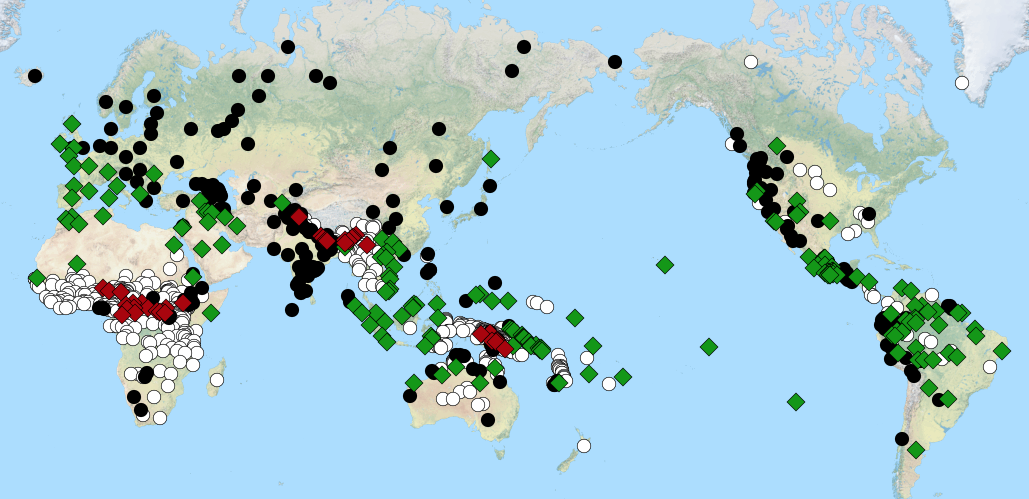
\includegraphics[width=1\textwidth]{./figures/NewU18Map.png}
\caption{Geographical distribution of ordering patterns based on \cite{wals-87,wals-89}. Circles are harmonic (black: Adj-N, \ili{Num}-N, white: N-Adj, N-\ili{Num}), diamonds are non-harmonic (green: N-Adj, \ili{Num}-N, red: Adj-N, N-\ili{Num}).}\label{fig: U18}
\end{figure}


Beyond Universal 18, Table \ref{table: U18} reveals a second trend in the raw frequency data: ordering patterns which place both Adj and \ili{Num} on the same side of the noun are by far the most common in the sample. This type of pattern is sometimes called\is{harmonic vs. non-harmonic} \is{typological universals} \textsc{harmonic}, while the other two are \textsc{non-harmonic} \citep[for discussion of this terminology see][59-62]{croft2003typology}. A trend toward harmony across phrases is a well known typological universal (many other Greenbergian universals are relevant for this, e.g., 2-6), which has been the subject of much research \citep[e.g.,][]{Hawkins83,Travis84,Chomsky88,Dryer92,Baker01}. To summarize then, we can hypothesize two biases based on these typological data: (i) a bias \is{biases} in favor of harmonic patterns, and (ii) a bias against the particular non-harmonic pattern combining pre-nominal adjectives with post-nominal numerals. 

\subsection{Testing Universal 18}
\is{learnability}
The four patterns in Table \ref{table: U18} are intuitively simple and are all clearly learnable. How, then, might one uncover potentially subtle \textit{differences} in learnability? In \cite{CulbertsonSmolenskyLegendre12} we did this by introducing variation into the input, essentially allowing us to see which patterns are more easily learnable under noisy conditions. Native-\ili{English}-speaking adult learners were trained on phrases comprised of a noun and single modifier (adjective or numeral word), the order of which varied between a dominant order--heard in 70\% of utterances--and the opposite--heard in 30\% of phrases. The dominant order varied randomly across participants in the experiment and instantiated one of the four possible patterns in Table \ref{table: U18}. The conditions are represented in Figure \ref{fig: U18conditions}, with numbers 1--4 indicating the four conditions. For example, in condition 1, learners heard pre-nominal Adj-N and \ili{Num}-N 70\% of the time, and post-nominal N-Adj, N-\ili{Num} the remaining 30\% of the time. Condition 2 has the opposite proportions, and therefore participants heard post-nominal N-Adj and N-\ili{Num} as the dominant order. Conditions 3 and 4 are non-harmonic; condition 3 participants heard N-Adj and \ili{Num}-N as the dominant pattern, while condition 4 participants heard the U18-violating Adj-N, N-\ili{Num} as the dominant pattern.

\begin{figure}
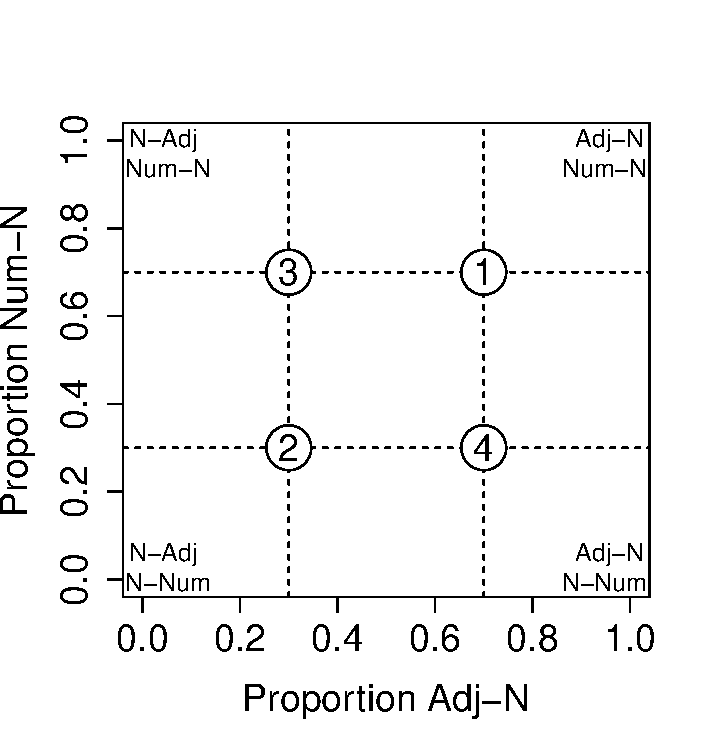
\includegraphics[width=0.5\textwidth]{figures/conditions}
\caption{Illustration of experiment conditions. The corners of this space represent deterministic patterns, while inset numbers represent the four variable conditions used in the experiment. Note that condition 1 and 2 are harmonic, while 3, 4 are non-harmonic. Condition 4 is a variable version of the U18-violating pattern.}\label{fig: U18conditions}
\end{figure}

Independent evidence from natural language and \is{artificial language learning} ALL studies \citep[e.g.,][]{SingletonNewport04,HudsonKamNewport09} suggests that learners tend to \textit{regularize} \is{regularization} unpredictable (unconditioned) variation of the sort we used in this experiment. We hypothesized that learners would be most likely to regularize variable patterns which conformed to their biases, \is{biases} and would not regularize those they found more difficult to learn. This predicts that participants learning a variable version of one of the two harmonic \is{harmonic vs. non-harmonic} patterns (1: Adj-N, \ili{Num}-N, or 2: N-Adj, N-\ili{Num}) should regularize the majority order, using it more than 70\% of the time. By contrast, participants learning the non-harmonic pattern targeted by Universal 18 (4: Adj-N, N-\ili{Num}) should \textit{not} regularize that pattern.

 


\begin{figure}
\begin{subfigure}[b]{0.45\textwidth}
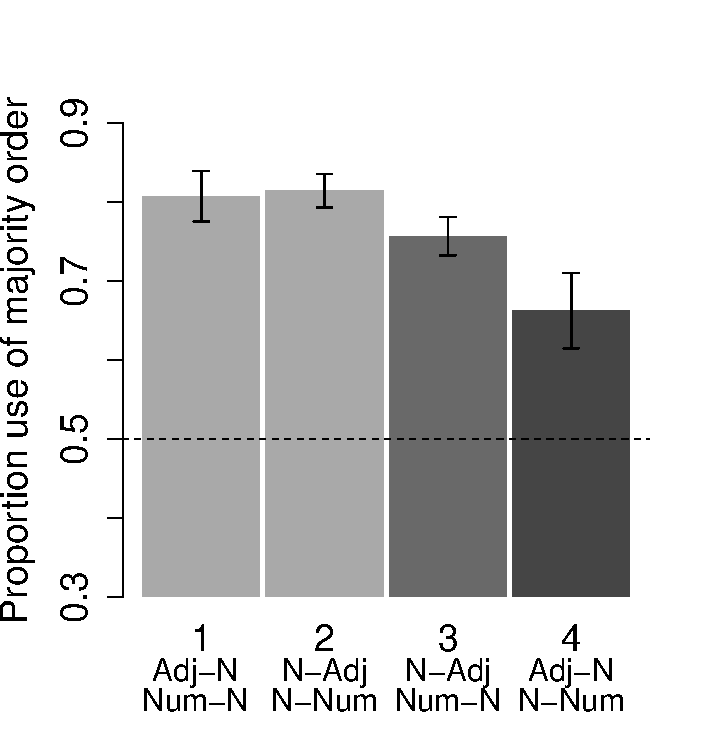
\includegraphics[height=.3\textheight]{figures/U18ResultsAverage}%
\caption{Average use of the majority order in each condition.\\}
\end{subfigure}
~~~~
\begin{subfigure}[b]{0.45\textwidth}
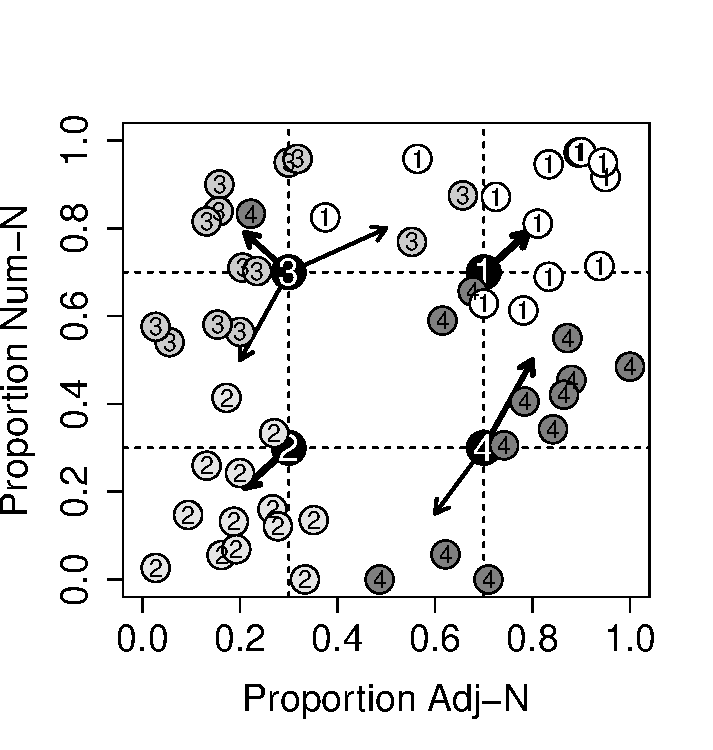
\includegraphics[height=.3\textheight]{figures/U18ResultsGSpace}
\caption{Behavioral outcomes for individual participants in each condition relative to their input.}
\end{subfigure}
\caption{Experiment results.}\label{fig: U18results}
\end{figure}


These predictions were borne out by the results, as shown in Figure \ref{fig: U18results}(a): participants in conditions 1 and 2 regularized the variation in their input--using the majority order substantially more than 70\% of the time--while participants in condition 4 did not regularize. Participants in condition 3, who were exposed to the non-harmonic pattern not violating U18, show some regularization but not as much as those in the harmonic conditions. Another way to visualize the behavioral outcomes in the experiment is in terms of the space shown in Figure \ref{fig: U18results}(b), which plots individual participants' use of each order relative to their input. This illustrates how learners \textit{shift} or change the language they are exposed to according to their biases. In conditions 1 and 2, learners' tendency to regularize aligns with their bias for harmonic patterns, therefore their output is shifted toward the deterministic corners relative to the input. In \is{harmonic vs. non-harmonic} non-harmonic condition 3, some learners shift toward a more regular version of their input, but others actively move the language toward one of the two preferred harmonic patterns. In non-harmonic condition 4, this shifting toward a harmonic pattern is much more dramatic and \textit{no} learners have regularized \is{regularization} their input pattern. Interestingly, in this experiment native \ili{English}-speaking \is{biases} participants showed only a small preference for their native-language order: the average regularization was the same across conditions 1 and 2, however more participants in the non-harmonic conditions shifted toward the pre-nominal harmonic pattern \citep[for additional discussion about prior language experience and an alternative explanation of this difference see][]{CulbertsonSmolenskyLegendre12, culbertson2015harmonic}.

To summarize, in \cite{CulbertsonSmolenskyLegendre12}, we started with Universal 18 and generated a set of hypothesized biases. We tested the psychological reality of these biases \is{biases} using an \is{artificial language learning} artificial language learning paradigm which exploits learners' tendency to regularize unpredictable variation. We confirmed that regularization of variation is indeed modulated by the particular type of pattern being learned; when the majority pattern in the input conforms to learners' biases, \is{biases} \is{regularization} they regularize. When the majority pattern is dispreferred, learners actively change the language to bring it in line with their preferences. With this evidence in hand, researchers interested in constructing explanations for the typological distribution of nominal word order can more confidently add these factors into their models. Moreover, additional research using experimental methods can begin to explore \textit{why} Universal 18 holds in the population tested, and \textit{why} learners might prefer harmonic patterns. This could involve testing structurally similar patterns in non-linguistic domains or investigating the role of language experience in the development of these biases.

\section{Greenberg's Universal 20}

\subsection{Introduction}

Greenberg's Universal 20 (U20), as reformulated by \cite{Cinque05}, is stated in (\ref{ex: U20}) below.

\begin{exe}
	\ex\label{ex: U20} In pre-nominal position: Dem-\ili{Num}-Adj
	\\
	In post-nominal position: Dem-\ili{Num}-Adj or Adj-\ili{Num}-Dem
\end{exe}

The explanation for this \is{implicational universals} implicational universal has received significant attention in the literature, particularly after additional typological work by \cite{Cinque05} and \cite{dryer2009order}. Figure \ref{fig: U20freq} plots the frequency of each of the 24 possible combinations of N, Dem, \ili{Num}, Adj in descending order. The two post-nominal orders picked out by Greenberg are highlighted in black. To account for this distribution, or key aspects it, a number of distinct proposals have been made \citep[e.g.,][]{Cinque05, abels2012linear, dryer2009order, cysouw2010dealing,SteddySamekLodovici11}. All of these proposals include a notion of the semantic or structural distinctions among the modifiers that can be described in terms of \textsc{scope}, \is{scope} as illustrated in Figure \ref{fig: U20hierarchy}. In this case, adjectives can be said to take innermost scope since they modify dimension inherent to noun meaning, while numerals serve to count these larger units. Demonstratives take highest scope because they serve to connect the internal material to the surrounding discourse. 

%\cite{Cinque05} posits an underlying hierarchical structure and a set of allowable movement operations in order to distinguish attested from unattested orders. \cite{dryer2009order} proposes an alternative set of violable principles to account for the frequency differences (including a harmony principle and a Universal 18 principle). \cite{cysouw2010dealing} uses regression modeling to show that three factors---harmony, a preference for post-nominal adjectives, and a particular structural configuration---provide a good fit to the typological data. The notion of structural configuration which \cite{cysouw2010dealing} uses is . 

\begin{figure}
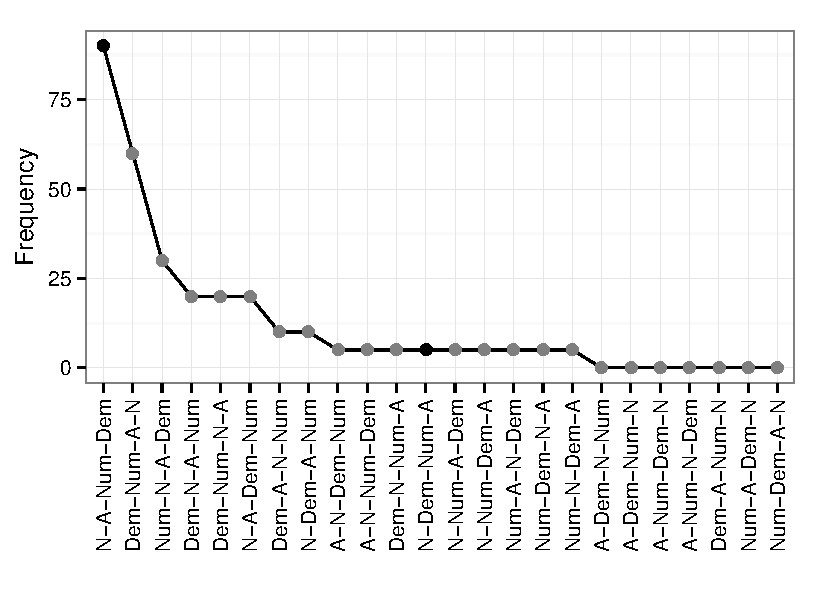
\includegraphics[width=0.9\textwidth]{figures/U20Freq}
\caption{Frequency of 24 possible combinations of N, Dem, \ili{Num}, Adj as reported in \cite{dryer2009order}. Post-nominal orders in Greenberg's Universal 20 are the black points.}\label{fig: U20freq}
\end{figure}

\begin{figure}

\begin{subfigure}[t]{.6\textwidth}
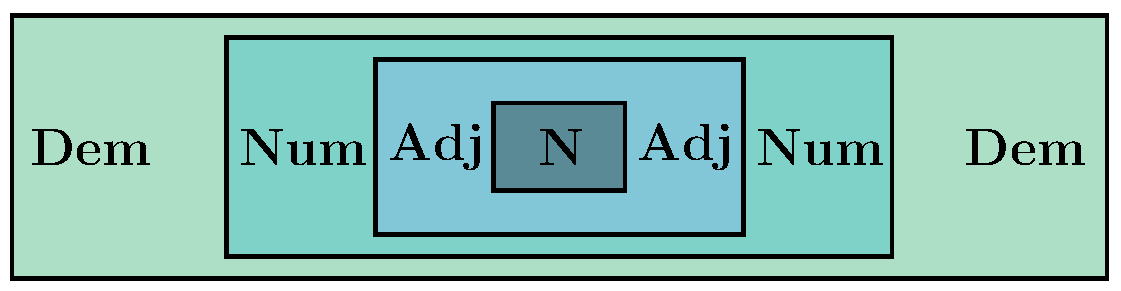
\includegraphics[width=\textwidth]{figures/ScopePic}
\caption{Illustration of nested scope relationship among nominal modifiers.}
\end{subfigure}
~~
\begin{subfigure}[t]{.3\textwidth}
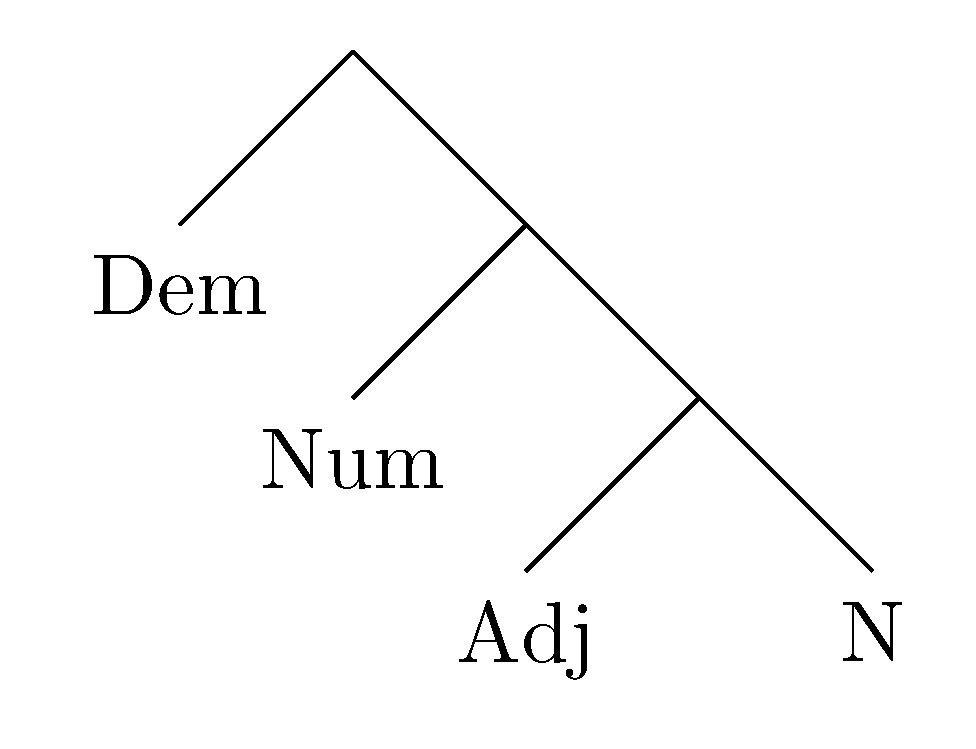
\includegraphics[width=\textwidth]{figures/tree1}
\caption{Hierarchical representation of scope. Dem takes widest scope, Adj takes innermost scope.}
\end{subfigure}
\caption{Scope relationship among nominal modifiers}\label{fig: U20hierarchy}
\end{figure}

These scope relations do not determine linear order, instead a given language can map these structural relations to linear order in various ways. Importantly, of the 24 possible patterns, eight preserve the underlying scope relations in the surface linear order. If in addition to preservation of the scope relations, harmony is also a factor which constrains language change, then we can explain why Dem-\ili{Num}-Adj-N and the mirror order N-Adj-\ili{Num}-Dem are the most frequent. Indeed, a principle encoding a harmony preference is present in most analyses of Universal 20, and harmonic patterns were shown to be preferred by learners in \cite{CulbertsonSmolenskyLegendre12}. By the same reasoning, the alternative post-nominal pattern cited by Greenberg, N-Dem-\ili{Num}-Adj, is expected to be less frequent since it is harmonic but does \textit{not} maintain the isomorphism between scope and the linear order.  \is{scope}

\subsection{Testing U20}
\is{typological universals} \is{poverty-of-the-stimulus}
The two post-nominal orders in Greenberg's Universal, N-Adj-\ili{Num}-Dem and N-Dem-\ili{Num}-Adj differ from one another in two important ways. First, as described above, N-Adj-\ili{Num}-Dem maintains the underlying scope relations in the linear order, while N-Dem-\ili{Num}-Adj does not (in fact it perturbs them maximally). Second, N-Dem-\ili{Num}-Adj has the same linear order of the modifiers as \ili{English}, while N-Adj-\ili{Num}-Dem does not (in fact it is the opposite). In \cite{culbertson2014language}, we capitalized on this pattern of differences to test whether \ili{English} speakers learning a new language will transfer their knowledge of linear order, or their knowledge of scope-to-surface isomorphism. We did this by using the \textsc{poverty-of-the-stimulus paradigm}, in which learners are presented with examples from a new language in a way that withholds critical evidence about its structure. At test, learners must generalize to held-out data that will disambiguate the alternative hypotheses. In this experiment, participants heard phrases with a noun and a single post-nominal modifier and then at test were asked about the relative order of modifiers. For example, they might be trained on N-Dem and N-Adj sequences, and then be asked at test whether phrases with N-Adj-Dem or N-Dem-Adj order are most likely in the language.

\begin{figure}

\begin{subfigure}[t]{.4\textwidth}

\parbox{.45\textwidth}{
\vspace*{-6cm}
\begin{tabular}{ll}
\lsptoprule
Training order & Testing combo\\
\midrule
N-Adj, N-Dem & \{Adj, Dem\}\\
N-\ili{Num}, N-Dem & \{\ili{Num}, Dem\}\\
N-Adj, N-\ili{Num} & \{Adj, \ili{Num}\}\\
\lspbottomrule 
\end{tabular}
}
\caption{Experimental conditions}
\end{subfigure}
~~~~
\begin{subfigure}[t]{.5\textwidth}
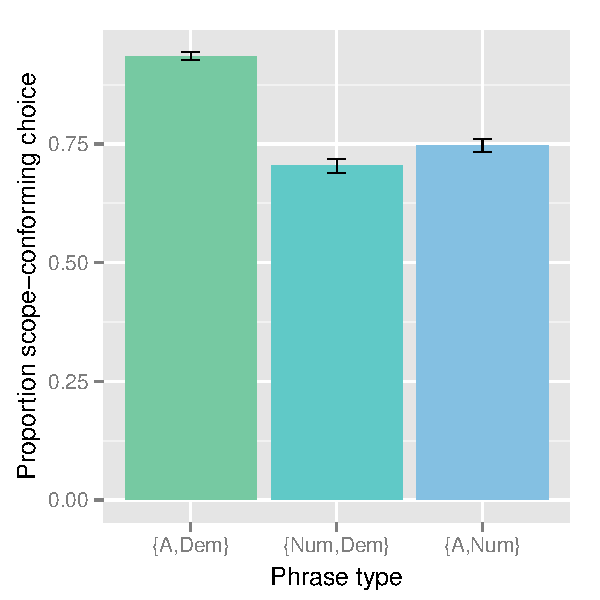
\includegraphics[width=1\textwidth]{figures/U20results}
\caption{Results by condition from Experiment 1}
\end{subfigure}

\caption{Conditions and results as reported in \cite{culbertson2014language}.}\label{fig: U20results}
\end{figure}

We trained participants in a number of different input conditions. Here I highlight one set, summarized in Figure \ref{fig: U20results}(a). The results, shown in Figure \ref{fig: U20results}(b), reveal a striking preference at test for orders which are isomorphic to the scope over those with are more surface-similar to \ili{English}. \is{scope} Interestingly, this preference was most dramatic when the input included Dem and Adj. This suggests that preserving the scope relations among the two most structurally distant modifiers (Dem and Adj) may be more important than the closer ones (either Dem, \ili{Num} or \ili{Num}, Adj). This prediction turns out to be typologically accurate; languages which perturb the scope of Adj, \ili{Num} or \ili{Num}, Dem are about twice as common as Adj, Dem.

To summarize, this result provides the first experimental evidence for a bias \is{biases} favoring linear orders that maintain an isomorphism with the underlying semantic scope. \is{scope} The evidence is preliminary to the extent that participants' bias \is{biases} may come from knowledge of this abstract property of \ili{English}. To determine whether the bias can be found in learners without direct experience with it, future work will need to target a population whose language \textit{violates} this preference--for example \ili{Kikuyu} is one of the few languages with N-Dem-\ili{Num}-Adj. Nevertheless, combined with a preference for harmony, as shown in \cite{CulbertsonSmolenskyLegendre12}, this provides a promising potential explanation for the typological asymmetry among these 24 ordering patterns. As with Universal 18, the scope of this bias remains an open question which can be investigated further using experimental techniques. It could be the case that the mapping between hierarchical structure and linear order in other domains (i.e. motor/action planning) respects similar kinds of constraints.

\section{Conclusion}
\is{typology} \is{generative linguistics} \is{human language faculty} \is{biases!soft}
Research in typology is critical for generative linguistics, where the enterprise is to characterize the human language faculty, including any constraints on the systems it can generate. Although there is disagreement as to whether these constraints must be hard-and-fast limits, or soft biases, and whether they are necessarily special features of language, typology is a source of crucial data. I have suggested here that these data should be used in formulating hypotheses about possible biases rather than treated as their observable result. Accordingly, the goal of much research using ALL paradigms is to provide behavioral evidence for hypothesized connections between typological patterns, like Greenberg's word order universals, \is{typological universals} \is{constituent order} and properties of the human cognitive system. The two case studies described above present examples of this kind of research; in both cases, biases are hypothesized on the basis of typological data, and predicted effects on learning are tested using ALL. \is{artificial language learning} These experiments corroborate the typological \is{typology} evidence, suggesting that (1) learners are biased in favor of harmonic word order patterns and disfavor one non-harmonic pattern especially (Adj-N, N-\ili{Num}), and (2) learners tend to infer relative orders of nominal modifiers that preserve the underlying semantic relations among them. \is{learnability} \is{functional typology}  \is{generative linguistics}

To the extent that connections between typological frequency and ease of learning are borne out, I would argue that the results also bear on major questions addressed by work in functionally-oriented typology; distinctions among patterns in terms of learnability (or use-ability) can be integrated into theories constructed to explain pathways of language change and, ultimately, typological distributions. The methods themselves are also increasingly used to further investigate the content and scope of biases, and whether they might be amplified or altered by social or communicative context. The case studies I have highlighted here illustrate, I hope, the kind of work that is informed by and can make progress in addressing important issues for both typology and generative linguistics.

%%%%Open question: linkage between biases and typology, how do we know that a given bias actually DID play a part in a given language history?
\section*{Acknowledgements}
I would like to thank Nick Enfield and attendees of the \textit{Dependencies Among Systems of Language} workshop, held June 2014 in Ardennes, Belgium. I also thank Larry Hyman for comments on a previous version of this paper.%\corref{cor1}
 
{\sloppy
\printbibliography[heading=subbibliography,notkeyword=this]
}

\end{document}  